\section{Messung des Stillstandsdrehmomentes}

\subsection{Beschreibung}

Im ersten Versuch soll die Momentenkonstante $k_m$ bestimmt werden.
Sie hängt folgendermaßen mit dem Drehmoment $M_M$ und dem Motorstrom
zusammen. 

\begin{equation} \label{eq1}
    \begin{split}
        M_M(t)&=k_m \cdot i_a(t)\\
        k_m&=\frac{M_M(t)}{i_a(t)}
    \end{split}
\end{equation}

Als Messwerte ist eine Matrix mit den Motorströmen $I_a$ und der Auslenkungskraft
$F$ gegeben. Um daraus das Drehmoment $M_M$ zu bestimmen wird der Radius $r$
benötigt, welcher mit $1 \mathrm{cm}$ gegeben ist.

\begin{equation} \label{eq2}
    \begin{split}
        M_M=f(I_a)&=r \cdot F(I_a)
    \end{split}
\end{equation}

Anschließend kann die Momentenkonstante $k_m$ über die Steigung der geplotteten
Gerade bestimmt werden. Hierfür muss gewährleistet werden, dass der Arbeistpunkt
linear ist. Deshalb dürfen die letzten drei Messwerte in der linearen Regression
nicht betrachtet werden.

\begin{equation} \label{eq3}
    \begin{split}
        k_m\simeq 0.022 \mathrm{\frac{Nm}{A}}
    \end{split}
\end{equation}


% \lipsum[1]\\




\subsection{Ausgabe der Lösung}
\begin{figure}[H]
 \centering
 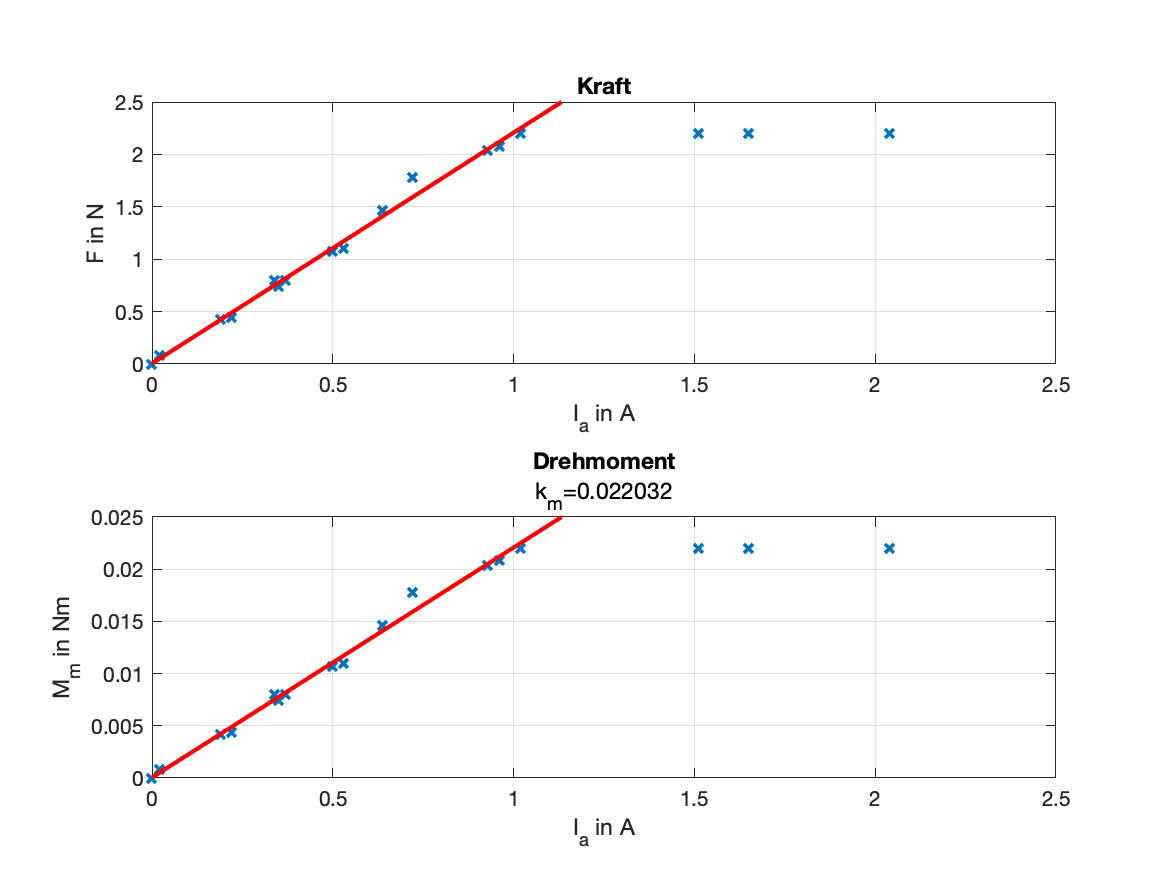
\includegraphics[width=1\textwidth]{as_labor01_1.png}
 \caption{Plot der Aufgabe 1}
 \label{fig:PlotAufgabe1}
\end{figure}

\subsection{Matlab Code}
\lstinputlisting[language=Matlab]{matlab/as_labor01_1.m}
